\section{Appendix sections}

 \begin{figure}[htp]
  \begin{center}
   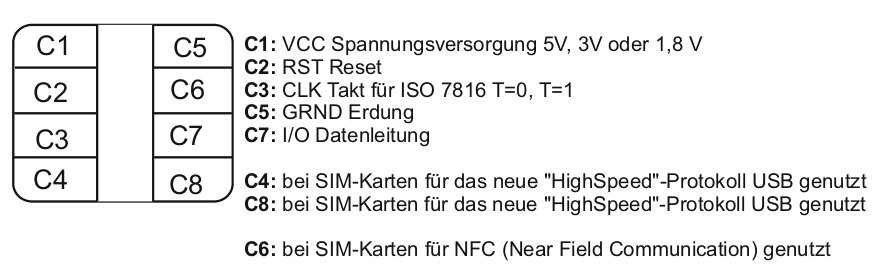
\includegraphics[width=410pt]{pinbelegung_chipkartensicherheit}
  \end{center}
  \caption[Pinbelegung einer Chipkarte]{Pinbelegung einer Chipkarte nach ISO/IEC 786 \cite{spitz11}}
  \label{abb:pinbelegung_chipkarten}
 \end{figure}

 \begin{figure}[htp]
  \begin{center}
   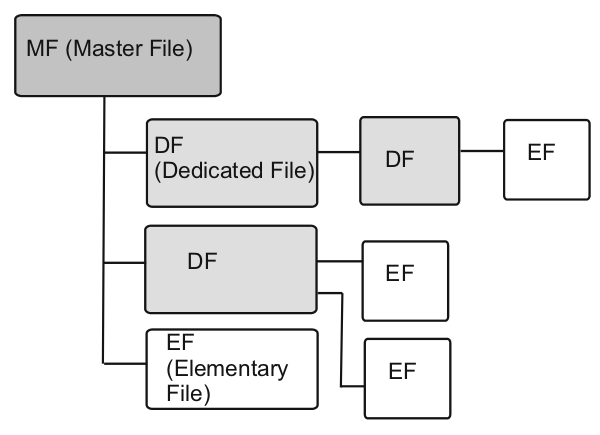
\includegraphics[width=350pt]{filesystem_chipkarten_chipkartensicherheit}
  \end{center}
  \caption[Filesystemarchitektur einer Chipkarte]{Filesystemarchitektur einer Chipkarte nach ISO/IEC 786 \cite{spitz11}}
  \label{abb:filesystem_chipkarten}
 \end{figure}

  \begin{figure}[htp]
  \begin{center}
   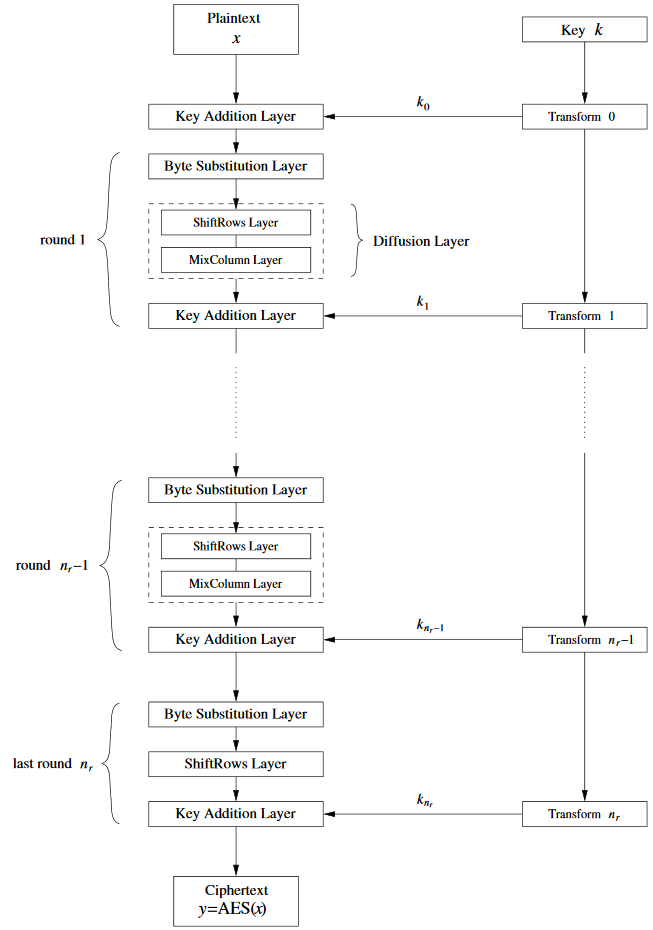
\includegraphics[width=440pt]{ablauf_aes}
  \end{center}
  \caption[Grafische Darstellung der AES-Verschlüsselung]{Grafische Darstellung der AES-Verschlüsselung \cite{paar10}}
  \label{abb:funktion_aes}
 \end{figure}
 
  \begin{figure}[htp]
  \begin{center}
   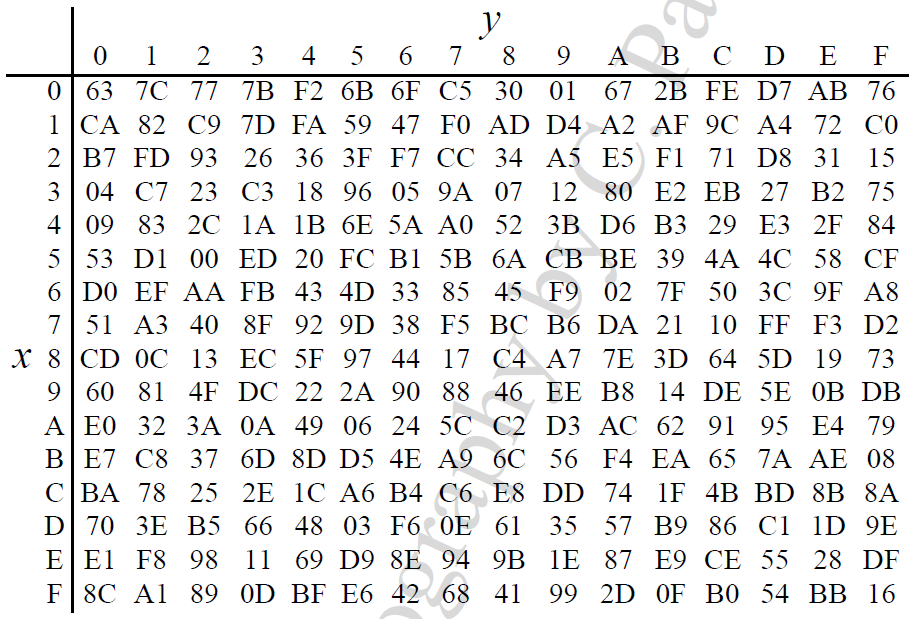
\includegraphics[width=440pt]{s-box}
  \end{center}
  \caption[Substitutionstabelle für AES-Verschlüsselung]{Substitutionstabelle für AES-Verschlüsselung \cite{paar10}}
  \label{abb:s-box}
 \end{figure}
 
 \begin{figure}[htp]
  \begin{center}
   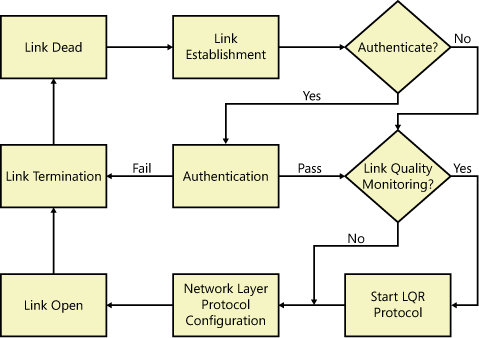
\includegraphics[width=350pt]{aufbauphasen_pppverbindung}
  \end{center}
  \caption[Aufbauphasen einer PPP-Verbindung]{Aufbauphasen einer PPP-Verbindung \cite{zackercomptia}}
  \label{abb:aufbauphasen_pppverbindung}
 \end{figure}

 \begin{figure}[htp]
  \begin{center}
   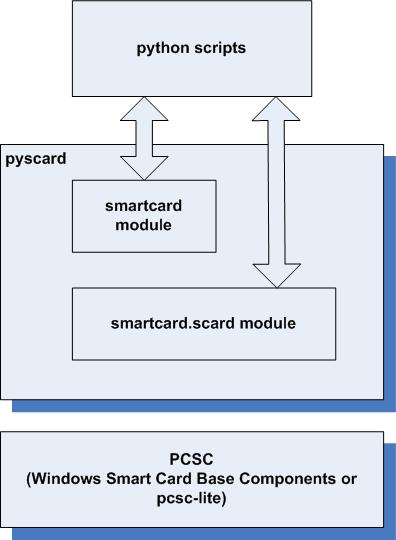
\includegraphics[width=350pt]{pyscard_schema}
  \end{center}
  \caption[Architektur der pyscard-Bibliothek]{Architektur der pyscard-Bibliothek \cite{pyscardweb}}
  \label{abb:pyscard_schema}
 \end{figure}